\textbf{Ejemplo 4}\\

Un proyecto requiere una inversión inicial de  COP  40.000, en el período 1 los ingresos son iguales a los egresos, en el período 2 hay un ingreso neto de  COP  100.000, en los períodos 3 y 4 los ingresos y los egresos vuelven a dar un flujo de caja neto de 0, finalmente en el período 5 hay un egreso de  COP  60.000. Calcular la TIR del proyecto. 
\\

\textbf{Solución.}\\
%La tabla ira centrada
\begin{center}
	\renewcommand{\arraystretch}{1.5}% Margenes de las celdas
	%Creación de la cuadricula de 3 columnas
\begin{longtable}[H]{|c|c|c|}
		%Creamos una linea horizontal
\hline
		%Definimos el color de la primera fila
\rowcolor[HTML]{FFB183}
%%%%% INICIO ASIGNACIÓN PERÍODO FOCAL %%%%%%%
  %%%%%%%%%% INICIO TITULO
  %Lo que se hace aquí es mezclar las 3 columnas en una sola
  \multicolumn{3}{|c|}{\cellcolor[HTML]{FFB183}\textbf{1. Asignación período focal}}   \\ \hline
  %%%%%%%%%% FIN TITULO
  %%%%% INICIO DECLARACIÓN DE VARIABLES %%%%%%%
  \multicolumn{3}{|c|}{$pf = 0 pmv$}   \\ \hline
  
%%%%%%%%%%% INICIO TITULO
\rowcolor[HTML]{FFB183}
\multicolumn{3}{|c|}{\cellcolor[HTML]{FFB183}\textbf{2. Declaración de variables}}    \\ \hline
%%%%%%%%%%% FIN TITULO
%%%%%%%%%%% INICIO MATEMÁTICAS

$\text{Inversión inicial} =  COP  40.000$                                     & \multicolumn{2}{c|}{$ i= COP  ? $} \\
$\text{Periodo 2 ingreso} =  COP  100.000 $	& \multicolumn{2}{c|}{$  $} \\
$ \text{Periodo 5 ingreso} =  COP  60.000 $	&	\multicolumn{2}{c|}{ $ $ } \\
$ n= 5 pmv $	&	\multicolumn{2}{c|}{ $ $ } \\ 
$  $	&	\multicolumn{2}{c|}{ $  $ }
\\
$  $	&	\multicolumn{2}{c|}{ $ $ }
\\
\hline
%%%%%%%%%% FIN MATEMÁTICAS
		%%%%% INICIO FLUJO DE CAJA
\rowcolor[HTML]{FFB183}
\multicolumn{3}{|c|}{\cellcolor[HTML]{FFB183}\textbf{3. Diagrama de flujo de caja}} \\ \hline
		%Mezclamos 3 columnas y pondremos el dibujo
		%%%%%%%%%%%%% INSERCIÓN DE LA IMAGEN
		%Deberán descargar las imágenes respectivas del drive y pegarlas en la carpeta
		%n_capitulo/img/ejemplos/1/capitulo1ejemplo1.pdf  (el /1/ es el numero del ejemplo)
\multicolumn{3}{|c|}{ 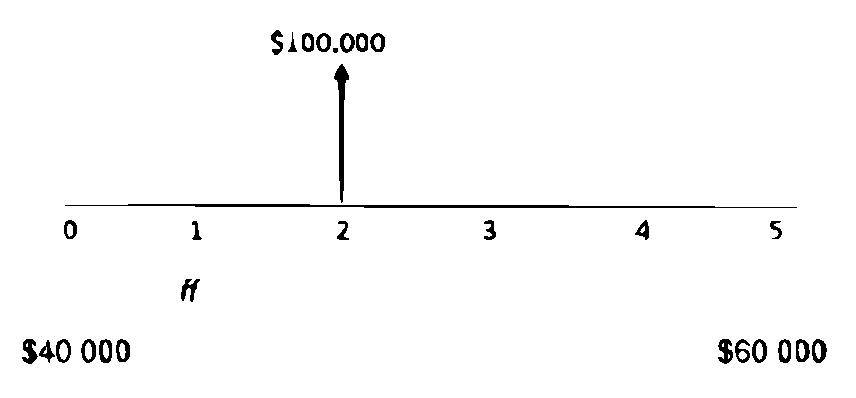
\includegraphics[scale=0.6, trim=-5 -5 -5 -5]{ejemplo5.pdf} }    
   \\\hline
		%%%%%%%%%%%%% FIN INSERCIÓN DE IMAGEN
		%%%%%FIN FLUJO DE CAJA
		
		
		
		%%%%% INICIO DECLARACIÓN FORMULAS
		%%%%%%%%%%% INICIO TITULO
\rowcolor[HTML]{FFB183}
\multicolumn{3}{|c|}{\cellcolor[HTML]{FFB183}\textbf{4. Declaración de fórmulas}}    \\ \hline
		%%%%%%%%%%% FIN TITULO
		%%%%%%%%%%% INICIO MATEMÁTICAS
\multicolumn{3}{|c|} {VPN =	$\sum F_{n}(1+i)^{-n}$   Valor presente neto.}   \\ 
\multicolumn{3}{|c|} { $ i= j/m $ }   \\ 

\hline	
	
		%%%%%%%%%% FIN MATEMÁTICAS
		%%%%%% INICIO DESARROLLO MATEMÁTICO
\rowcolor[HTML]{FFB183}
		%%%%%%%%%%INICIO TITULO
\multicolumn{3}{|c|}{\cellcolor[HTML]{FFB183}\textbf{5. Desarrollo matemático}}       \\ \hline
		%%%%%%%%%% FIN TITULO
		%%%%%%%%%% INICIO MATEMÁTICAS
		\multicolumn{3}{|c|}{$ —  COP  40.000 +  COP  100.000(1+1)^{-2} —  COP  60.000(1+1)^{-5} =  COP  0 $}  
		\\
		
		\multicolumn{3}{|c|}{$ \text{Construimos una tabla de valores X,Y para ver el comportamiento} $}  
		\\
		\multicolumn{3}{|c|}{$ \text{de la gráfica y así determinar las tasas} $}  
		\\	
		\multicolumn{3}{|c|}{ 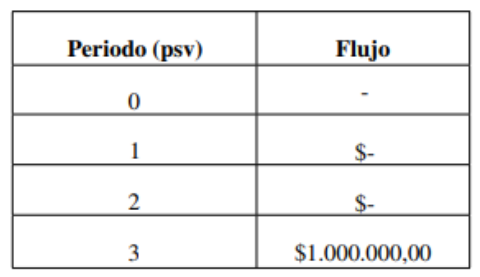
\includegraphics[scale=1, trim=-5 -5 -5 -5]{tabla.png} }    
		\\
		\multicolumn{3}{|c|}{ $\frac{39\%-40\%}{39\%-x} = \frac{193.976-(-135.658)}{193.975-0} $ }  
		\\
		\multicolumn{3}{|c|}{$ \text{Suponiendo una tasa del 30\% para la reinversión, los ingresos serán:} $}  
		\\
		\multicolumn{3}{|c|}{$  COP  100.000(1 + 0.3)^{3}=  COP  219.700 $}  
		\\
		\multicolumn{3}{|c|}{$  COP  40.000 +  COP  60 000(1+0.25)^{-5} =  COP  59.660.80 $}  
		\\
		\multicolumn{3}{|c|}{$ \text{El nuevo diagrama de flujo de caja es:} $}  
		\\
		\multicolumn{3}{|c|}{ 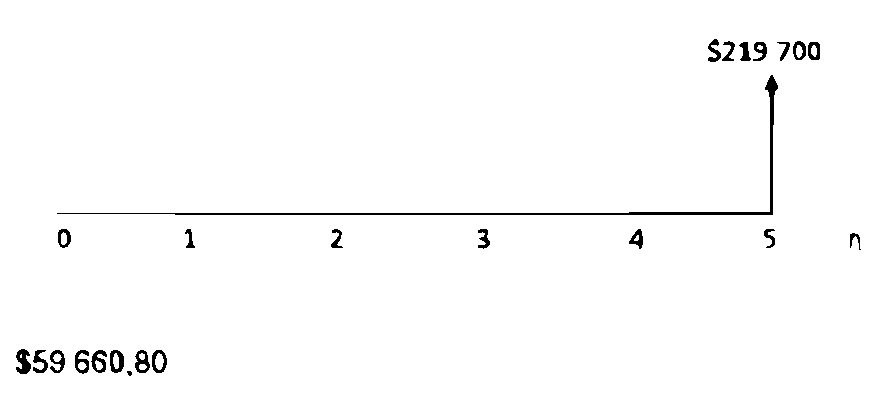
\includegraphics[scale=1, trim=-5 -5 -5 -5]{ejemplo52.pdf} }    
		\\
		\multicolumn{3}{|c|}{$  COP  219.700 =  COP  59.660,80(1+i)^{5} $}  
		\\
		\multicolumn{3}{|c|}{$ TIRM = i = 29.786\% pmv $}  
		\\
	    \hline
				
		%%%%%%%%%% FIN MATEMÁTICAS
		%%%%%% FIN DESARROLLO MATEMÁTICO
		%%%%%% INICIO RESPUESTA
\rowcolor[HTML]{FFB183}
		%%%%%%%%%%INICIO TITULO
\multicolumn{3}{|c|}{\cellcolor[HTML]{FFB183}\textbf{6. Respuesta}}   \\ \hline
		%%%%%%%%%% FIN TITULO
		%%%%%%%%%% INICIO RESPUESTA MATEMÁTICA
		
\multicolumn{3}{|c|}{ \text{Esta tasa se debe comparar con la TIO para tomar una decisión. Vale la pena anotar que no es por una}}
\\
\multicolumn{3}{|c|}{\text{simple manipulación matemática que el proyecto rinda el 29.78\% pmv. Desde el punto de vista financiero } }
\\
\multicolumn{3}{|c|}{\text{es mejor recibir  COP  100.000 en 2 pmv que recibir  COP  40.000 ahora y  COP  60.000 en 5 pmv. } }
\\
\hline

		
		%%%%%%%%%% FIN MATEMÁTICAS
		%%%%%% FIN RESPUESTA
	\end{longtable}
	%Se crean dos lineas en blanco para que no quede el siguiente texto tan pegado
	%\newline \newline %USARLO SI CREES QUE ES NECESARIO
\end{center}
%%%%%%%%%%%%%%%%%%%%%%%%%%FIN EJERCICIO 1 %%%%%%%%%%%%%%%%%%%%%%%%%%%


\textbf{}\\
